\graphicspath{{cpeg1/}}


\chapter{Atmospheric Entry Guidance}
\label{sec:cpeg1}

As scientific and crewed payloads have more demanding goals, precise atmospheric entry guidance is playing an increasing role in mission success. State-of-the-art entry guidance algorithms are structured in a predictor-corrector framework, where a simulation is used to predict a trajectory, and corrections are then made to the control inputs.  These guidance methods are simple and effective, but current algorithms assume low lift-to-drag entry vehicles, are limited to only bank-angle control, and have a limited ability to guarantee the safety of the vehicle. We propose a new predictor-corrector entry guidance method that formulates the correction step as a convex optimization problem. This allows for more flexibility in specifying the vehicle's dynamics and control inputs, and the ability to explicitly handle safety constraints such as heating, pressure, and acceleration limits. We test the new algorithm in Mars entry scenarios similar to the Mars Science Laboratory with both bank-angle control and bank-angle plus angle-of-attack control, demonstrating both its performance and ability to generalize to future vehicle capabilities.

The contents of this chapter have been previously published at IEEE Aerospace Conference 2021 in \citet{tracy2022c}

%%%%%%%%%%%%%%%%%%%%%%%%%%%%%%%%%%%%%%
\section{Introduction}
%%%%%%%%%%%%%%%%%%%%%%%%%%%%%%%%%%%%%%
In 1971 the Soviet Union's Mars-2 spacecraft made history by entering the Martian atmosphere before impacting the surface.  Nine days later, an identical Mars-3 spacecraft performed the first soft-landing on the Martian surface, ushering in a new era in planetary exploration. NASA followed with successful Mars landings in 1976 with Viking 1 and 2 and has since then landed and operated multiple robotic systems on the Martian surface \cite{li2014}. 

Entry vehicle architectures can be divided into three broad categories \cite{li2014}: 1) Ballistic entry is an uncontrolled descent with drag as the only force, 2) unguided ballistic-lifting entry has an uncontrolled non-zero lift force, and 3) guided ballistic-lifting entry has some control over the vehicle's lift vector. Controlled entry guidance allows for the prioritization of landing locations with scientific merit instead of just those that minimize risk to the vehicle.

The Mars Science Laboratory (MSL) carrying the Curiosity rover touched down in 2012 as the first Mars entry vehicle with guided ballistic-lifting entry.  MSL had control over the vehicle bank angle during entry, enabling control of the direction of the lift vector within the lifting plane. While MSL dramatically reduced the size of the landing ellipse from over 100 km to 10 km, its guidance is still too coarse for pinpoint landings. By developing more performant entry guidance capabilities, entry vehicles could effectively place robotic or crewed landers in desirable science collection areas, including high altitude sites. 

% \section{Previous Work}
Much of the work on guidance for low lift-to-drag entry vehicles originated with the Apollo terminal guidance methods. These algorithms, as described in \cite{graves1972}, rely on control of the bank angle with simple switching manuevers to control the cross-range and down-range errors. Slightly modified versions have been developed for use with more recent Mars entry vehicles, such as in \cite{mendeck2014}.  Current research investigates the use of predictor-corrector algorithms \cite{brunner2012} to improve the landing accuracy. A popular predictor-corrector formulation that exhibits bank-angle switching behavior is the Fully Numerical Predictor-corrector Entry Guidance (FNPEG) algorithm \cite{lu2008}. In the baseline FNPEG algorithm, Newton's method is used to solve for a static bank-angle that satisfies a terminal downrange distance constraint, and the sign of the bank-angle is modulated to control crossrange errors \cite{lu2014}. Here, the prediction phase is used to generate gradients for the terminal constraint, and corrections are applied to the open-loop commanded bank-angle in an effort to satisfy these terminal constraints. This framework is simple and effective but requires significant added complexity for incorporation of safety constraints or changes to the vehicle control inputs.

Trajectory optimization for offline planning of entry vehicle trajectories has been explored in \cite{wang2016} and \cite{wang2018a}, where the nonconvex optimal control problem was solved by linearizing the nonlinear dynamics and constraints, solving a conic optimization problem with a trust region, and repeating until convergence. This successive-convexification method was used instead of standard NonLinear Programming (NLP) solvers, like SNOPT \cite{gill2005} or IPOPT \cite{wachter2006}, because it is able to directly handle second-order cone constraints instead of relying on local linear approximations. Optimal trajectories computed offline were then paired with an optimization-based tracking controller, as described in \cite{wang2016} and \cite{wang2018a}. While these formulations are able to stabilize a trajectory, there are no guarantees that safety constraints can be satisfied online. Also, the computational complexity of the trajectory-optimization formulation makes these methods intractable for real-time control onboard an entry vehicle.

The Convex Predictor-corrector Entry Guidance (CPEG) algorithm proposed in this paper combines ideas from trajectory optimization with the predictor-corrector guidance framework by solving a constrained optimization problem during the correction step.  First, the dynamics of the entry vehicle with the current control plan are simulated to a target altitude for a predicted trajectory. Next, the vehicle dynamics are linearized about the predicted trajectory and a convex trajectory optimization problem is solved that minimizes landing error. By solving for a correction using convex optimization, CPEG is able to reason about the full state and control history to inform the correction instead of just the final state.  This also allows for the vehicle's safety constraints, such as heating, pressure, and acceleration, to be explicitly included in the correction computation. Our specific contributions in this paper are:
\begin{enumerate}
    \item A general quasi-linear formulation of entry vehicle dynamics that is well-suited to numerical optimization.
    \vspace{8pt}
    \item A predictor-corrector entry guidance algorithm with a highly generalizable correction step utilizing convex optimization.
    \vspace{8pt}
    \item Customized trust regions and objective functions for entry vehicles with multiple control modalities. 
\end{enumerate}

The paper proceeds as follows: In Section \ref{sec:cpeg1:dynamics}, the classic Vinh entry vehicle dynamics are compared with a more modern Cartesian approach. In Section \ref{sec:cpeg1:trajopt}, the details of the full nonconvex trajectory optimization problem are discussed. In Section \ref{sec:cpeg1:cpeg}, the CPEG algorithm is derived. In Section \ref{sec:cpeg1:experiments}, CPEG is validated on entry vehicles with bank-angle control, as well as bank-angle and angle-of-attack control. Finally, Section \ref{sec:cpeg1:conclusion} outlines our conclusions and potential future research directions.


\section{Entry Vehicle Dynamics}
\label{sec:cpeg1:dynamics}

Despite much of the recent powered-descent guidance literature using Cartesian state representations, entry vehicles are still most often represented in spherical coordinates. In this section, the traditional entry vehicle dynamics denoted below as the ``Vinh'' model will be discussed, as well as an alternative Cartesian formulation. 

\subsection{The Vinh Model}
The classic Vinh model, presented in 1976 in \cite{busemann1976} and again a few years Later in Vinh's textbook \cite{vinh1980}, has been the standard method for simulating entry vehicles for the past 45 years. Parameterizing the entry vehicle in spherical coordinates, the state in the Vinh model contains familiar terms like latitude, longitude, and flight-path angle. Despite being highly nonlinear and prone to scaling issues, it is the most common dynamics model in the literature \cite{busemann1976,vinh1980,vinh2000,wang2018,wang2019a,lu2014,gallais2007}.

The dynamics in the Vinh model are calculated with the angle-of-attack, $\alpha$, bank-angle, $\sigma$, flight-path angle, $\gamma$, longitude, $\theta$, latitude, $\phi$, and heading angle, $\psi$. The resulting equations of motion over a planet that's rotating with a constant angular velocity $\Omega$ are,
\begin{align}
\dot{r}&=V \sin \gamma ,\label{eq:vin1}\\
\dot{\theta}&=V \cos \gamma \sin \psi /(r \cos \phi) ,\\
\dot{\phi}&=V \cos \gamma \cos \psi / r ,\\
\dot{V}&=-D-\sin \gamma / r^{2} +\Omega^{2} r \cos \phi\sin \gamma \cos \phi   -\Omega^{2} r \cos \phi \cos \gamma \sin \phi \cos \psi  ,\\
\dot{\gamma}&=L \cos \sigma / V+\left(V^{2}-1 / r\right) \cos \gamma /(V r) +2 \Omega \cos \phi \sin \psi +\Omega^{2} r \cos \phi\cos \gamma \cos \phi / V   
 \\ & \quad \quad + \Omega^{2} r \cos \phi\sin \gamma \sin \phi \cos \psi / V , \\
\dot{\psi}&=L \sin \sigma /(V \cos \gamma)+V \cos \gamma \sin \psi \tan \phi / r 
 -2 \Omega(\tan \gamma \cos \psi \cos \phi-\sin \phi) \\ 
  & \quad \quad +\Omega^{2} r \sin \phi \cos \phi \sin \psi /(V \cos \gamma) , \label{eq:vin6}
\end{align}
where $r$ is the normalized radial distance from the center of the planet, $V$ is the normalized planet-relative velocity, and L and D are the magnitudes of the lift and drag accelerations. 

This model is highly nonlinear in both the state and the control, even when the planetary motion is ignored. While the planet's angular velocity is assumed to be constant, its inclusion in the dynamics still contributes significant nonlinearities. Because of this, much of the literature ignores the planet's angular velocity \cite{wang2016}. There are also scaling issues present if these equations are naively implemented. Since $r$ and $V$ are not angles, they are usually of a much larger magnitude than the rest of the state. This can lead to poor accuracy in variable time-step integrators, as well as ill-conditioning in numerical trajectory optimization.

\subsection{Cartesian Entry Dynamics}
We have found that entry vehicle dynamics are both simpler to derive and numerically better-conditioned when represented in standard Cartesian coordinates instead of the spherical coordinates used in the Vinh formulation. This state representation is popular with the powered-descent guidance community, albeit without any aerodynamic forces in the dynamics \cite{blackmore2012, acikmese2007, acikmese2013}.

We assume a planet-fixed frame $P$ is aligned with an inertial frame $N$ along the $z$ axis. The planet spins with angular velocity $\omega \in {\mathbb{R}}^3$ in the positive $z$ direction, making the velocity of the entry vehicle the following:
\begin{align}
{}^P v  &= {}^N v  -    \omega  \times r, \label{eq:pv}
\end{align}
where $^Nv \in {\mathbb{R}}^3$ is the inertial velocity, $^Pv \in {\mathbb{R}}^3$ is the planet relative velocity, and $r \in {\mathbb{R}}^3$ is the position of the entry vehicle in the planet frame. This expression can be differentiated once more to provide the relationship between the inertial and planet-relative accelerations:
\begin{align}
{}^P a &=   {}^{N} a -       2( \omega \times {}^P v )                          -   \omega  \times (\omega \times r) .\label{eq:Pa}
\end{align}
The state of the entry vehicle can be parameterized with the planet-relative position vector $r$, and planet relative velocity ${}^P v$ denoted as just $v$, both expressed in the coordinates of the planet frame. The Cartesian dynamics can now be written in state space as,
\begin{align}
    {\begin{bmatrix} v \\ a \end{bmatrix}} &= \begin{bmatrix} 0 & I \\ -[\omega \times]^2 & -2[\omega \times] \end{bmatrix}\begin{bmatrix}r \\v  \end{bmatrix} + \begin{bmatrix} 0 \\  a_{g} + a_{D} + a_{L} \end{bmatrix},\label{eq:dynamics}
\end{align}
where $[\omega \times]$ is the skew-symmetric cross product matrix,
\begin{align}
    [\omega \times ] &= \begin{bmatrix} 0 &-\omega_3 &\omega_2 \\ 
                                     \omega_3 &0 & -\omega_1 \\ 
                                     -\omega_2 & \omega_1 & 0 \end{bmatrix}.
\end{align}
One of the main benefits of the dynamics in equation \eqref{eq:dynamics} is the linear kinematics. This means that linear approximations of the relationship between position and velocity are exact, and the only nonlinearities present are in the accelerations. The gravitational acceleration in the direction of the planet's center is expressed assuming simple spherical gravity:
\begin{align}
    a_g &= -\frac{\mu}{\|r\|^3}r,
\end{align}
 where $\mu \in \mathbb{R}$ is the standard gravitational constant for the given planet. The acceleration caused by the drag force is in the direction opposing velocity, and is calculated as,
\begin{align}
    a_D &= - \frac{1}{2m}\rho A C_d \|v\| v,
\end{align}
where $m \in \mathbb{R}$ is the mass of the entry vehicle, $\rho \in \mathbb{R}$ is the atmospheric density, $A \in \mathbb{R}$ is the aerodynamic reference area, and $C_d \in \mathbb{R}$ is the coefficient of drag.  In this work, the atmospheric density $\rho \in \mathbb{R}$ will be represented by a piecewise exponential function \cite{gallais2007}.

\begin{figure}[t]
    \centering
    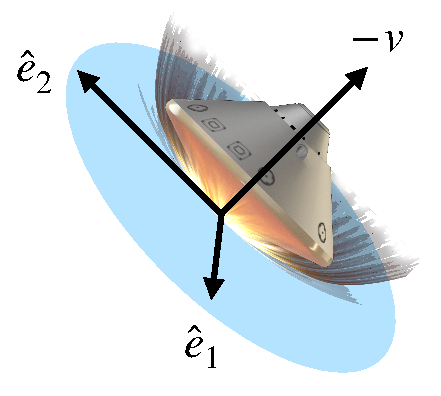
\includegraphics[width = 2in]{burn.pdf}
    \caption{The $E$ frame is fixed to the entry vehicle, with $\hat{e}_1$ in the direction of the specific angular momentum vector, and $\hat{e}_2 = \hat{v} \times \hat{e}_1$. When defined in this frame, the lift vector can be expressed using only $\hat{e}_1$ and $\hat{e}_2$.}
    \label{fig:eframe}
\end{figure}

For the description of the lift acceleration, a reference frame is defined that describes a plane about the entry vehicle that is orthogonal to the velocity vector.  This two-dimensional frame, referred to as the $E$ frame and depicted in Fig. \ref{fig:eframe}, has two basis vectors described by the following:
\begin{align}
    \hat{e}_1 &=  \frac{r \times v}{\|r \times v\|}, \\ 
    \hat{e}_2 &= \frac{v \times \hat{e}_1}{\| v \times \hat{e}_1 \|} .
\end{align}
The magnitude of the lift vector is calculated as,
\begin{align}
    \|L\| &= \frac{1}{2m} C_L \rho(r) A \|v\|^2,
\end{align}
where $C_L \in \mathbb{R}$ is the coefficient of lift. In the case where the entry vehicle only has control over the bank-angle, the resulting lift acceleration can be described by the magnitude of the lift and the bank-angle:
\begin{align}
    a_L &= \|L\|(\sin(\sigma)\hat{e}_1 + \cos(\sigma)\hat{e}_2). \label{eq:bao}
\end{align}
 In the case where the entry vehicle can control both the angle-of-attack as well as the bank-angle, the lift vector can be written as,
\begin{align}
    a_L &= \|L\|(\ell_1\hat{e}_1 + \ell_2\hat{e}_2), \label{eq:fl}
\end{align}
subject to the constraint $||\ell_1^2 + \ell_2^2|| \leq 1$.
Here the lift acceleration is a linear function of the control inputs, which is a key feature when this model is linearized in an optimization problem. Both the Vinh model and the Cartesian model are nonlinear, but the Cartesian model behaves significantly better under linearization, making it a far better candidate for trajectory optimization.


\subsection{State and Control Definitions}
In the case where only the bank-angle is controlled, the state is augmented with the bank-angle, and the sole control input is the derivative of this bank-angle with respect to time. This allows for cost functions that specify desired behavior for the derivative of the bank-angle, with the state and control as the following:
\begin{align}
x &= \begin{bmatrix} r^T & v^T & \sigma \end{bmatrix} ,\\ 
u &= \dot{\sigma}.
\end{align}
These dynamics are now in control-affine form with linear kinematics.  For the case with actuation of both the bank angle and angle-of-attack, the state and control are the following:
\begin{align}
x &= \begin{bmatrix} r^T & v^T \end{bmatrix}^T ,\\ 
u &= \begin{bmatrix} \ell_1 & \ell_2 \end{bmatrix}^T,
\end{align}
where $\ell_1$ and $\ell_2$ were defined in \eqref{eq:fl}. 
\section{Trajectory Optimization}
\label{sec:cpeg1:trajopt}
Feedback control laws for entry vehicles suffer in performance due to the severe underactuation of the vehicle. This is, in part, due to the fact that an entry vehicle has very limited ability to speed up or slow down in the along-track direction. To deal with this, it makes more sense to solve the guidance problem with a holistic planning approach, one that can reason about this limited control authority and plan for it. Therefore, we pose this problem as a trajectory optimization problem, where a locally optimal state trajectory and control plan can be solved for numerically.
%  \subsection{Reachable Set}
%  \todo{i kinda want to delete this section}
%  Given a bank-angle with a maximum angle-of-attack, the entry vehicle is able to control its final landing spot for the parachute deployment. To validate the dynamics model and view the possible places that the entry vehicle could deploy the parachute given this maximum allowable angle-of-attack, a set of simulations were run such that all of the possible bank-angles were sampled. The resulting plot is available in figure \ref{fig:reachable_set}, and is also known as the "landing footprint". This plot demonstrates that the entry vehicle does not have full controllabilty of the state and can't stabilize about a given trajectory, but it is able to fully articulate the spot in which the vehicle reaches an altitude of 10 km for the parachute deployment. This is critical because the objective of this control law is not to drive the state to a goal state at a goal time, but rather simply control the point in which the parachute system is deployed. 
% \begin{figure}
%     \centering
%     \includegraphics{tikz_figz/footprint.tikz}
%     \caption{Visualized reachable set for entry vehicle trajectories with only bank-angle control. Presented is a top view of 100 trajectories with varying bank-angle, each trajectory terminates at an altitude of 10 km.}
%     \label{fig:reachable_set}
% \end{figure}
 \subsection{Safety Constraints}
 Three key vehicle safety constraints --- heating, pressure, and acceleration --- are most dependent on the atmospheric density. Unfortunately, this is also the part of the environment in which there is the largest amount of uncertainty. The atmospheric density is often only known to roughly within a factor of two, with even less known about the wind conditions \cite{gallais2007}.
 
 The heating constraint has to do with the max allowable heat rate that the ablative heat shield can withstand \cite{edquist2007}. This is measured in power per square centimeter, and it is expressed as the following:
 \begin{align}
     \dot{Q} = k_q \sqrt{\rho}V^{3.15} \leq \dot{Q}_{max}. \label{eq:con_heat}
 \end{align} 
 This function is nonlinear but can be locally approximated with linear functions during the correction step.  The next safety constraint is the maximum dynamic pressure on the entry vehicle, which is expressed as the following:
 \begin{align}
     q = .5 \rho V^2 \leq q_{max}.\label{eq:con_press}
 \end{align}
 The last safety constraint is the maximum allowable normal load, which is the total aerodynamic force on the entry vehicle. This is expressed as a norm of the lift and drag forces:
 \begin{align}
     a = \sqrt{\|L\|^2 + \|D\|^2} \leq a_{max}.\label{eq:con_load}
 \end{align}
\subsection{Full Nonconvex Formulation}

In order to formulate a convex correction problem, we first consider the full nonlinear non-convex problem. First, the dynamics described in equation \eqref{eq:dynamics} are discretized with an explicit integrator like the classic fourth-order Runge-Kutta method \cite{montenbruck2002}, giving a discrete-time dynamics model of the form,
\begin{align} \label{eq: discrete-dynamics}
    x_{k+1} &= f(x_k,u_k,\Delta t_k).
\end{align}
No assumptions have been made about the control configuration in this dynamics model: it can account for either bank-angle-only or bank-angle plus angle-of-attack control. The full nonlinear trajectory optimization problem has the form,
% \begin{mini!} \label{nlp}
% {x,u,\Delta t}{x}{}{}
% %   {x,u,\Delta t}{\ell_N(x_N, u_N)+ \sum_{k=1}^{N-1}\ell_k(x_k, u_k) }{}{}
% %   \addConstraint{x_{k+1}}{= f(x_k,u_k,\Delta t_k),}{\forall k}
% %   \addConstraint{g_k(x_k, u_k)}{\leq 0,}{\forall k}
% %   \addConstraint{\Delta t_{min} \leq \Delta t_k }{\leq \Delta t_{max} }{\forall k}
% %   \addConstraint{x_N}{=x_{goal}}{},
% \end{mini!}
\begin{mini}<b>
  {x,u,\Delta t}{\ell_N(x_N, u_N)+ \sum _{k=1}^{N-1}\ell_k(x_k, u_k) }{}{}
  \addConstraint{x_{k+1}}{= f(x_k,u_k,\Delta t_k)}{\forall k} \labelOP{nlp}%\tag{test}
  \addConstraint{g_k(x_k, u_k)}{\leq 0}{\forall k} 
  \addConstraint{\Delta t_{min} }{\leq \Delta t_k \leq \Delta t_{max} }{\forall k}
  \addConstraint{x_N}{=x_{goal}}{},
 \end{mini}
 where safety constraints \eqref{eq:con_heat}---\eqref{eq:con_load} are included in the inequality constraint function $g_k(x_k, u_k)$. Note that this is a free-final-time problem in which the $\Delta t_k$ are decision variables in addition to the states and controls. This is necessary due to the inability of the entry vehicle to reach its goal state at an arbitrarily specified time. Problem \eqref{nlp} is nonconvex due to both the nonlinear dynamics, as well as the variable time between knot points. It is worth noting that, even with linear continuous-time dynamics, the discrete-time dynamics constraints \eqref{eq: discrete-dynamics} become nonlinear when the time step is made to be a decision variable.
 %This time step variable is bounded between two positive values to ensure the dynamics progress forward, and the dynamics don't take larger steps than is appropriate given the accuracy of the integrator. 
 
 Trajectory optimization problems like \eqref{nlp} can be solved with a variety of methods. One standard approach is to use an off-the-shelf NLP solver like IPOPT \cite{wachter2006} or SNOPT \cite{gill2005}. Alternatively, more specialized trajectory optimizers like ALTRO can be used \cite{howell2019,jackson2021}.  While computationally tractable using one of the described methods, the nonconvexity of the problem means there are no available guarantees for the quality of the solution or convergence of the solver. As a result, running nonconvex trajectory optimization onboard safety-critical aerospace systems is unpopular, explaining the prevalence of simpler heritage methods for entry guidance. 

 \section{Convex Predictor-corrector}
\label{sec:cpeg1:cpeg}
CPEG combines ideas from numerical trajectory optimization with the classic predictor-corrector guidance framework: It uses a prediction step, in which the vehicle dynamics are simulated until a target altitude is reached, combined with a corrector step that is based on solving a local convex approximation of a nonlinear trajectory optimization problem to steer the vehicle to the desired target. These steps are then repeated until convergence is achieved. This section provides a detailed derivation of the CPEG algorithm.

\subsection{Prediction and Dynamics Linearization}

In the first stage of CPEG, the dynamics of the entry vehicle are simulated with a standard Runge-Kutta method using the current nominal control trajectory, $\bar{U}$, until a target altitude is reached. We denote this predicted trajectory by $\bar{X}$. After the prediction step, the discrete-time nonlinear dynamics are approximated using a first-order Taylor series,
\begin{align}
    \bar{x}_{k+1} + \delta x_{k+1} \approx f(\bar{x}_k,\bar{u}_k) + A_k \delta x_k + B_k \delta u_k,
\end{align}
where $A_k$ and $B_k$ are the following Jacobians,
\begin{align}
    A_k &= \frac{\partial f(x_k,u_k,\Delta t_k)}{\partial x_k} \bigg\rvert _{\bar{x}_k,\bar{u}_k}, \label{jacob1}\\
    B_k &= \frac{\partial f(x_k,u_k,\Delta t_k)}{\partial u_k}\bigg\rvert _{\bar{x}_k,\bar{u}_k}. \label{jacob2}
\end{align}
Subtracting the dynamics of the reference trajectory from both sides, the local linear dynamics of trajectory corrections can be written as:
\begin{align}
    \delta x_{k+1} = A_k \delta x_k + B_k \delta u_k.\label{eq:linmod}
\end{align}
A crucial distinction between CPEG and sequential convexification methods \cite{wang2016,malyuta2021,mao2019}, is that trajectory iterates are always dynamically feasible, thanks to the prediction step. This eliminates the possibility of inconsistent linearizations of the dynamics constraints \cite{nocedal2006}, in which no feasible correction trajectory exists. Specifically, there is always a trivial solution to \eqref{eq:linmod} of all zeros for $\delta x$ and $\delta u$.

\subsection{Cost Function}
The cost function used in CPEG is comprised of a term that penalizes the miss distance from the target and a term that penalizes specified control behaviors. For the penalty on miss distance, putting a naive quadratic cost on the error between the final position and the desired position is inappropriate since it also penalizes altitude errors. Instead, only the position error projected onto the landing plane is penalized, effectively ignoring altitude error. Since the altitude target is implicitly satisfied during the prediction step, this allows for the correction to only apply changes to the control plan that minimize the projected miss distance. The cost function for this projected miss distance is the following:
\begin{align}
\ell_{miss}(\delta X,\delta U) &= \|W( r_N + \delta r_N - r_{goal})\|_2^2 ,\label{eq:miss}
\end{align}
where $r_N \in {\mathbb{R}}^3$ is the  final position in the reference trajectory, $\delta r_N \in {\mathbb{R}}^3$ is the correction computed for this position, and $r_{goal} \in {\mathbb{R}}^3$ is the desired final position for parachute deployment. To project this error onto the landing plane, we define following projection matrix, 
\begin{align}
W &= I - pp^T,
\end{align}
where $p$ is the unit vector normal to the planetary surface at the target position:
\begin{align}
p &= \frac{r_{goal}}{\|r_{goal}\|}.
\end{align}
The second part of the cost function seeks to shape the control behavior. In the case of bank-angle control, we consider two different control cost functions that produce qualitatively different behavior:
\begin{align}
    \ell_{\sigma,L1}(\delta U) &= \lambda \|\dot{\sigma_k}\|_1, \label{eq:bankl1}
\end{align}
and
\begin{align}
    \ell_{\sigma,quad}(\delta U) &= \lambda \dot{\sigma_k}^2, \label{eq:bankl2}
\end{align}
where $\lambda$ is a scalar tuning parameter. The first cost function \eqref{eq:bankl1} penalizes the L1 norm of the derivative of the bank-angle, resulting in bank-angle trajectories with a minimum number of discrete switches. The second cost function \eqref{eq:bankl2} penalizes the square of the bank-angle derivative, resulting in smooth bank-angle trajectories. For the bank-angle plus angle-of-attack case, as described in \eqref{eq:fl}, we apply a simple quadratic cost to the norm of the controlled lift vector, effectively penalizing high angles of attack:
\begin{align}
    \ell_{\sigma \alpha}(\delta U) &= \lambda \|u_k\|_2^2. \label{eq:baoa_cost}
\end{align}
\subsection{Constraints}
Of the three nonlinear safety constraints, two can be linearized, and the third can be converted to a conservative convex relaxation. For the heating and dynamic pressure constraints \eqref{eq:con_heat}--\eqref{eq:con_press}, a Taylor expansion of each is formed, approximating the constraint to first-order. From here, a linearized inequality constraint can be directly included in the convex correction problem. For these constraints, the linearized versions are:
\begin{align}
 [\nabla \dot{Q}(\bar{x}_k)]^T \delta x_k &\leq \dot{Q}_{max} - \dot{Q}(\bar{x}_k), \label{eq:lincon_heat}\\ 
  [\nabla {q}(\bar{x}_k)]^T \delta {x}_k &\leq {q}_{max} - {q}(\bar{x}_k). \label{eq:lincon_press}
\end{align}
The acceleration loading constraint \eqref{eq:con_load} is nonlinear, but a conservative convex relaxation can be derived in the form of a second-order cone constraint. First, the kinematics for the velocity can be conservatively approximated as the following:
\begin{align}
v_{k+1} &= v_k + a_k \Delta t, \\ 
a_k &= \frac{v_{k+1} - v_k}{\Delta t}, \\
a_k &=  \frac{\bar{v}_{k+1} + \delta v_{k+1} - \bar{v}_k - \delta v_k}{\Delta t}.
\end{align}
The maximum loading constraint can then be re-written as,
\begin{align}
% \|a_k\|_2 = \frac{1}{\Delta t} \|\bar{v}_{k+1} + \delta v_{k+1} - \bar{v}_k - \delta v_k\| &\leq a_{max} \\
 \|\bar{v}_{k+1} + \delta v_{k+1} - \bar{v}_k - \delta v_k\| &\leq  \Delta t \cdot a_{max}, \label{eq:lincon_accel}
\end{align}
which is in the form of a convex second-order cone, and can be directly incorporated into the correction problem.

The three  safety constraints from equations \eqref{eq:lincon_heat}, \eqref{eq:lincon_press}, and \eqref{eq:lincon_accel}, are stacked into a generic safety constraint function, 
\begin{align}
g_{safety}(\delta x_k, \delta u_k) &\leq 0 . 
\end{align}
\subsection{Trust Region}
To ensure that corrections are sufficiently small that the dynamics linearizations and constraint approximations remain accurate, a trust-region constraint is added to the convex correction problem. While standard trust-region methods apply norm constraints to $\delta  X$ and $\delta U$ \cite{nocedal2006}, insight into the entry guidance problem enables a more tailored approach. 

The quality of the linearization presented in \eqref{eq:linmod} is highly accurate for approximating the vehicle kinematics, gravity, and atmospheric drag, but is much less accurate when applied to the bank-angle in the bank-angle-only control case. Therefore, we design a trust region that restricts corrections to the bank-angle, $\delta \sigma_k$, given the known accuracy of small-angle approximations but allows large corrections to the other states. This approach also allows us to avoid the need to adapt trust regions inside the solver, enabling faster and more reliable convergence. We apply the following trust-region constraints to each corrector problem:
\begin{align}
\|\delta u_k\|_2 &\leq \delta u_{max}\\
|\delta \sigma_k | &\leq \delta \sigma_{max}
\end{align}
\subsection{Convex Corrector Problem}
For the case where the entry vehicle has control of only the bank-angle as described in \eqref{eq:bao}, the convex correction problem can be formulated as,
\begin{mini}
  {\delta X, \delta U}{\ell_{miss}(\delta X, \delta U) + \ell_{\sigma }(\delta U)}{\label{cpeg_boa}}{}
  \addConstraint{A_k \delta x_k + B_k \delta u_k}{=\delta x_{k+1}}{}
  \addConstraint{g_{safety}(\delta x_k, \delta u_k)}{\leq 0}{}
  \addConstraint{\|\delta u_k\|_2}{\leq \delta u_{max}}{}
  \addConstraint{|\delta \sigma_k |}{\leq \delta \sigma_{max},}{}
 \end{mini}
where the miss cost function is described in \eqref{eq:miss}, and the bank-angle cost function can be either \eqref{eq:bankl1} or \eqref{eq:bankl2}.

For the case where the entry vehicle has control over both bank-angle and angle-of-attack as described in \eqref{eq:fl}, the convex correction problem can be posed as:
\begin{mini}
  {\delta X, \delta U}{\ell_{miss}(\delta X, \delta U) + \ell_{\sigma \alpha}(\delta U)}{\label{cpeg_fl}}{}
  \addConstraint{A_k \delta x_k + B_k \delta u_k}{=\delta x_{k+1}}{}
  \addConstraint{g_{safety}(\delta x_k, \delta u_k)}{\leq 0}{}
  \addConstraint{\|u_k + \delta u_k\|_2}{\leq 1.}{} 
 \end{mini}
%A key difference here is that there is now a unit norm constraint on $u + \delta u$, ensuring the normalized lift control input does not exceed the maximum allowable lift.

These problems can be solved quickly and reliably by standard conic solvers such as Mosek \cite{mosekaps2014}, COSMO \cite{garstka2020}, and ECOS \cite{domahidi2013}.
%The trust region constraints ensure that the solution to this problem is within a reasonable region of linearization, allowing for the correction to be applied to the control plan with confidence.
 \subsection{CPEG Algorithm}
 The full CPEG algorithm is detailed in algorithm \ref{alg:flight}. The inputs to CPEG are the current position and the current control plan. From here, the dynamics of the entry vehicle are simulated until parachute deployment with the current control plan. This predicted trajectory is then discretized and linearized, resulting in dynamics Jacobians $A_k$ and $B_k$ (equations \eqref{jacob1}-\eqref{jacob2}). From here, the convex correction problem is posed given the control configuration and cost strategy. This convex optimization problem is solved, and the correction $\delta U$ is used to correct the control plan. The prediction-correction steps are repeated until the norm of the correction being made to the control plan is below a specified tolerance. 
  \begin{algorithm} 
	\begin{algorithmic}[1]
		\caption{CPEG Algorithm}\label{alg:flight}
		\State \textbf{input} $x_0$, U  \Comment{nominal control plan}
		\While{$\|\delta U\| > $ tolerance}
    		\State $\Bar{X}, \Bar{U} = \text{simulate}(x_0,U)$ \Comment{predict trajectory}
    		\State $A,B = \text{linearize}(\Bar{X}, \Bar{U})$ \Comment{linearize about prediction}
    		\State $\delta X,\delta U = \text{cvx}(\Bar{X}, \Bar{U}, A, B)$ \Comment{solve for correction} 
    	    \State $U \mathrel{+}= \delta U $ \Comment{correct control plan}
		\EndWhile
		\State \textbf{return} $U$ \Comment{return updated control plan}
	\end{algorithmic}
\end{algorithm}

\section{Numerical Experiments}
 \label{sec:cpeg1:experiments}
Parameters roughly matching those of the Mars Science Laboratory (MSL) \cite{mendeck2014} were used to test the CPEG algorithm. All scenarios begin at an altitude of $125$ km above the Martian surface with a Mars-relative velocity of 5.845 km/second. CPEG was implemented in the Julia programming language \cite{bezanson2017}, using the Convex.jl optimization modeling library \cite{udell2014}, and the Mosek \cite{mosekaps2014} and OSQP \cite{stellato} solvers. CPEG was validated on the following three cases:
\begin{itemize}
    \item Bank-angle control with L1 cost penalty, denoted $\sigma_{L1}$.
    \vspace{+2mm}
    \item Bank-angle control with quadratic penalty, denoted $\sigma_{2}$.
    \vspace{+2mm}
    \item Bank-angle plus angle-of-attack control, denoted $\sigma + \alpha$.
\end{itemize}
For the bank-angle cases, CPEG was arbitrarily initialized with a constant bank-angle of zero, with noise added to the bank-angle derivative. For the bank-angle plus angle-of-attack case, a similar approach was used, but noise was added to the normalized lift vector. The final converged trajectories for the three cases are shown in figures \ref{fig:allalt} and \ref{fig:allcrdr}. In all of the cases, CPEG was able to successfully guide the entry vehicle to the target point at the desired altitude.
\begin{figure}
    \centering
    \includegraphics{cpeg1/tikz/all_altdr.tikz}
    \caption{Altitude and downrange distance from the converged trajectories from CPEG on the three specified cases. The $\sigma_{L1}$ case is with bank-angle control and an L1 penalty on bank-angle derivative, $\sigma_{quad}$ is bank-angle only with a quadratic penalty on bank-angle derivative, and $\sigma + \alpha$ is control over both bank-angle and angle-of-attack. Due to the differences in control authority and cost function, all three converge on different trajectories that hit the target position at parachute deployment.}
    \label{fig:allalt}
\end{figure}
% \todo{Describe what the different cases are in all of the figure captions as well (i.e. spell out what the labels mean).}
\begin{figure}
    \centering
    \includegraphics{cpeg1/tikz/all_crdr.tikz}
    \caption{Crossrange and downrange trajectory data from the converged trajectories from CPEG on the three specified cases. The cases with only control over the bank-angle have to do a bank reversal to hit the target, whereas the case with control over bank-angle and angle-of-attack is able to leverage the full lift control to avoid the switching.}
    \label{fig:allcrdr}
\end{figure}
\subsection{Bank-Angle Control}
For the case where the entry vehicle has only bank-angle control, the convergence of CPEG can be observed in figures \ref{fig:l1alt} and \ref{fig:l1crdr} for the case with an L1 cost on the bank-angle derivative, and figures \ref{fig:l2alt} and \ref{fig:l2crdr} with a quadratic cost.  These plots show the output of the prediction step of CPEG, where the color of the predictions is blue for the first iteration of the algorithm and turns purple, then pink for later iterations.
\begin{figure}
    \centering
    \includegraphics{cpeg1/tikz/L1_altdr.tikz}
    \caption{Predicted entry vehicle trajectories for the bank-angle only L1 penalty case, as seen by the altitude and downrange data. As the iterates continue, the entry vehicle converges on a trajectory that reaches the target at the 10km altitude mark.} 
    \label{fig:l1alt}
\end{figure}
\begin{figure}
    \centering
    \includegraphics{cpeg1/tikz/L1_crdr.tikz}
    \caption{Predicted entry vehicle trajectories for the bank-angle only L1 penalty case, as seen by the crossrange and downrange data.}
    \label{fig:l1crdr}
\end{figure}
  \begin{figure}
    \centering
    \includegraphics{cpeg1/tikz/L2_altdr.tikz}
    \caption{Predicted entry vehicle trajectories for the bank-angle only quadratic penalty case, as seen by the altitude and downrange data. The}
    \label{fig:l2alt}
\end{figure}
\begin{figure}
    \centering
    \includegraphics{cpeg1/tikz/L2_crdr.tikz}
    \caption{Predicted entry vehicle trajectories for the bank-angle only quadratic penalty case, as seen by the crossrange and downrange data.}
    \label{fig:l2crdr}
\end{figure}
After convergence, the two bank-angle profiles that CPEG produced for the L1 and quadratic cost functions are shown in figure \ref{fig:banks}. The L1 cost on the derivative of the bank-angle encouraged sparsity in this derivative, resulting in a bank-angle profile that switches between constant bank-angles. For the case with a quadratic cost on the bank-angle derivative, the resulting bank-angle profile is smooth with no discrete switching behavior.
\begin{figure}
    \centering
    \includegraphics{cpeg1/tikz/banks.tikz}
    \caption{Bank-angle only control plans for both the L1 and quadratic cost cases. The L1 cost motivated a bang-bang switching style bank-angle profile. The quadratic cost resulted in a smooth and continuous bank-angle profile.}
    \label{fig:banks}
\end{figure}
\subsection{Bank-Angle and Angle-of-Attack Control}
As described by the dynamics in equation \eqref{eq:fl}, the control input for this case is the lift vector itself in the directions orthogonal to the velocity vector. This allows for manipulation of both the bank-angle and angle-of-attack and is guaranteed to be within the maximum allowable lift by the unit norm constraint in equation \eqref{cpeg_fl}. In this control case, the control input Jacobian is constant and independent of the nominal control plan, making the linearization significantly more accurate than the bank-angle-only case. As a result, the convergence of CPEG with bank-angle plus angle-of-attack control is significantly faster than with the bank-angle alone. The evolution of the predicted trajectories is shown in figures \ref{fig:flalt} and \ref{fig:flcrdr}, with the same coloring scheme as the bank-angle only section. After convergence, the control inputs were converted back into bank-angle and angle-of-attack and shown together in figure \ref{fig:flcontrols}.
\begin{figure}
    \centering
    \includegraphics{cpeg1/tikz/FL_altdr.tikz}
    \caption{Predicted entry vehicle trajectories for the bank-angle and angle-of-attack case, as seen by the altitude and downrange data.}
    \label{fig:flalt}
\end{figure}
\begin{figure}
    \centering
    \includegraphics{cpeg1/tikz/FL_crdr.tikz}
    \caption{Predicted entry vehicle trajectories for the bank-angle and angle-of-attack case, as seen by the crossrange and downrange data.}
    \label{fig:flcrdr}
\end{figure}
\begin{figure}
    \centering
    \includegraphics{cpeg1/tikz/fl_controls.tikz}
    \caption{Bank-angle and angle-of-attack profiles for the case where both angles are being controlled. CPEG was able to converge on this control plan in just three iterations.}
    \label{fig:flcontrols}
\end{figure}
\section{Conclusion}
\label{sec:cpeg1:conclusion}
This paper proposes an improved version of the classic predictor-corrector entry guidance scheme in which the correction step is formulated as a convex optimization problem. Two control strategies were tested with CPEG: bank-angle control, and bank-angle plus angle-of-attack modulation. For the bank-angle-only case, cost functions that penalized the derivative with an L1 cost and a quadratic cost were both demonstrated, resulting in dramatically different optimal bank-angle profiles. For the case with both bank-angle and angle-of-attack control, the quality of the dynamics linearization was accurate enough that CPEG was able to converge on an optimal trajectory in just a few iterations. An implementation of CPEG running all of the examples in this paper is available at \url{https://github.com/RoboticExplorationLab/EntryGuidance.jl}.